\documentclass[twoside,twocolumn]{article}

\usepackage{blindtext} 
\usepackage{graphicx}
\usepackage[sc]{mathpazo} 
\usepackage[T1]{fontenc} 
\linespread{1.05} 
\usepackage{microtype} 

\usepackage[utf8]{inputenc} 


\usepackage[spanish,english]{babel} 



\usepackage[hmarginratio=1:1,top=32mm,columnsep=20pt]{geometry} 
\usepackage[hang, small,labelfont=bf,up,textfont=it,up]{caption} 
\usepackage{booktabs} 


\usepackage{lettrine} 


\usepackage{enumitem} 
\setlist[itemize]{noitemsep} 


\usepackage{abstract} 
\renewcommand{\abstractnamefont}{\normalfont\bfseries} 
\renewcommand{\abstracttextfont}{\normalfont\small\itshape} 


\usepackage{titlesec} 
\renewcommand\thesection{\Roman{section}} % 
\renewcommand\thesubsection{\roman{subsection}} 
\titleformat{\section}[block]{\large\scshape\centering}{\thesection.}{1em}{} 
\titleformat{\subsection}[block]{\large}{\thesubsection.}{1em}{} 


\usepackage{fancyhdr} 
\pagestyle{fancy} 
\fancyhead{} 
\fancyfoot{} 
\fancyhead[C]{Patrones de Diseño $\bullet$ Octubre 2020 $\bullet$ } 
\fancyfoot[RO,LE]{\thepage} 


\usepackage{titling} 


\usepackage{hyperref} 


%----------------------------------------------------------------------------------------
%	TILULOS
%----------------------------------------------------------------------------------------


\setlength{\droptitle}{-4\baselineskip} 

\pretitle{\begin{center}\Huge\bfseries} 
\posttitle{\end{center}} 
\title{Patrones de Diseño} 
\author{Percy Taquila Carazas, Katerin Merino Quispe}
\date{\today} 
\renewcommand{\maketitlehookd}{

\selectlanguage{english}
\begin{abstract}
\noindent 
Design patterns provide a coded mechanism for describing problems and their solution in a way that allows the software engineering community to design knowledge for reuse.
A pattern describes a problem, indicates the context and allows the user to understand the environment in which the problem occurs, and lists a system of forces that indicate how the problem can be interpreted in context, and the way in which the problem is applied. solution.
The Abstract Factory pattern is usually implemented with manufacturing methods that are also generally called from within the Template Method.
\end{abstract}


\selectlanguage{spanish}
\begin{abstract}
\noindent 
Los patrones de diseño dan un mecanismo codificado para describir problemas y su solución en forma tal que permiten que la comunidad de ingeniería de software diseñe el conocimiento para que sea reutilizado.
Un patrón describe un problema, indica el contexto y permite que el usuario entienda el ambiente en el que sucede el problema, y enlista un sistema de fuerzas que indican cómo puede interpretarse el problema en su contexto, y el modo en el que se aplica la solución.
El patron Abstract Factory suele implementarse con metodos de fabricacion que tambien generalmente son llamados desde el interior de Template Method.
\end{abstract}

}

%----------------------------------------------------------------------------------------

\begin{document}

% Print the title
\maketitle

%----------------------------------------------------------------------------------------
%	INTRODUCCION
%----------------------------------------------------------------------------------------

\section{Introduccion}

\lettrine[nindent=0em,lines=3]{E}l aprendizaje es esencial para la mayoría de las arquitecturas de redes neuronales, por lo que la elección de un algoritmo de aprendizaje es un punto central en el desarrollo de una red, este implica que una unidad de procesamiento es capaz de cambiar su comportamiento entrada/salida
como resultado de los cambios en el medio.\\

El camino hacia la construccion de maquinas inteligentes comienza en la Segunda Guerra Mundial con el diseÑo de computadoras analogicas ideadas para controlar cañones antiaereos o para la navegacion.
Algunos investigadores observaron que existıan semejanzas entre el funcionamiento de estos dispositivos de control y los sistemas reguladores de los seres vivos. De este modo, combinando los avances de la electronica de la posguerra y los conocimientos sobre los sistemas nerviosos de los seres vivos, inicio el reto de construir maquinas capaces de responder y aprender como los animales.




%----------------------------------------------------------------------------------------
%	Objetivos
%----------------------------------------------------------------------------------------


\section{Desarrollo}
En el aprendizaje supervisado debemos aprender a entrenar a la neurona, haciendo uso de ecuaciones matemáticas, para balancear sus pesos

A diferencia del aprendizaje supervisado, en el no supervisado solo se le otorgan las características, sin proporcionarle al algoritmo ninguna etiqueta. Su función es la agrupación, por lo que el algoritmo debería catalogar por similitud y poder crear grupos, sin tener la capacidad de definir cómo es cada individualidad de cada uno de los integrantes del grupo.



%----------------------------------------------------------------------------------------
%	Conclusiones
%----------------------------------------------------------------------------------------


\section{Conclusiones}

Los patrones de diseño dan un

%----------------------------------------------------------------------------------------
%	Recomendaciones
%----------------------------------------------------------------------------------------

\section{Recomendaciones}


\begin{itemize}
\item Cuando se conoce el efecto colateral que conlleva el patrón de diseño y es viable la aparición de este efecto.
\item Suministrar alternativas de diseño para poder tener un software flexible y reutilizable.


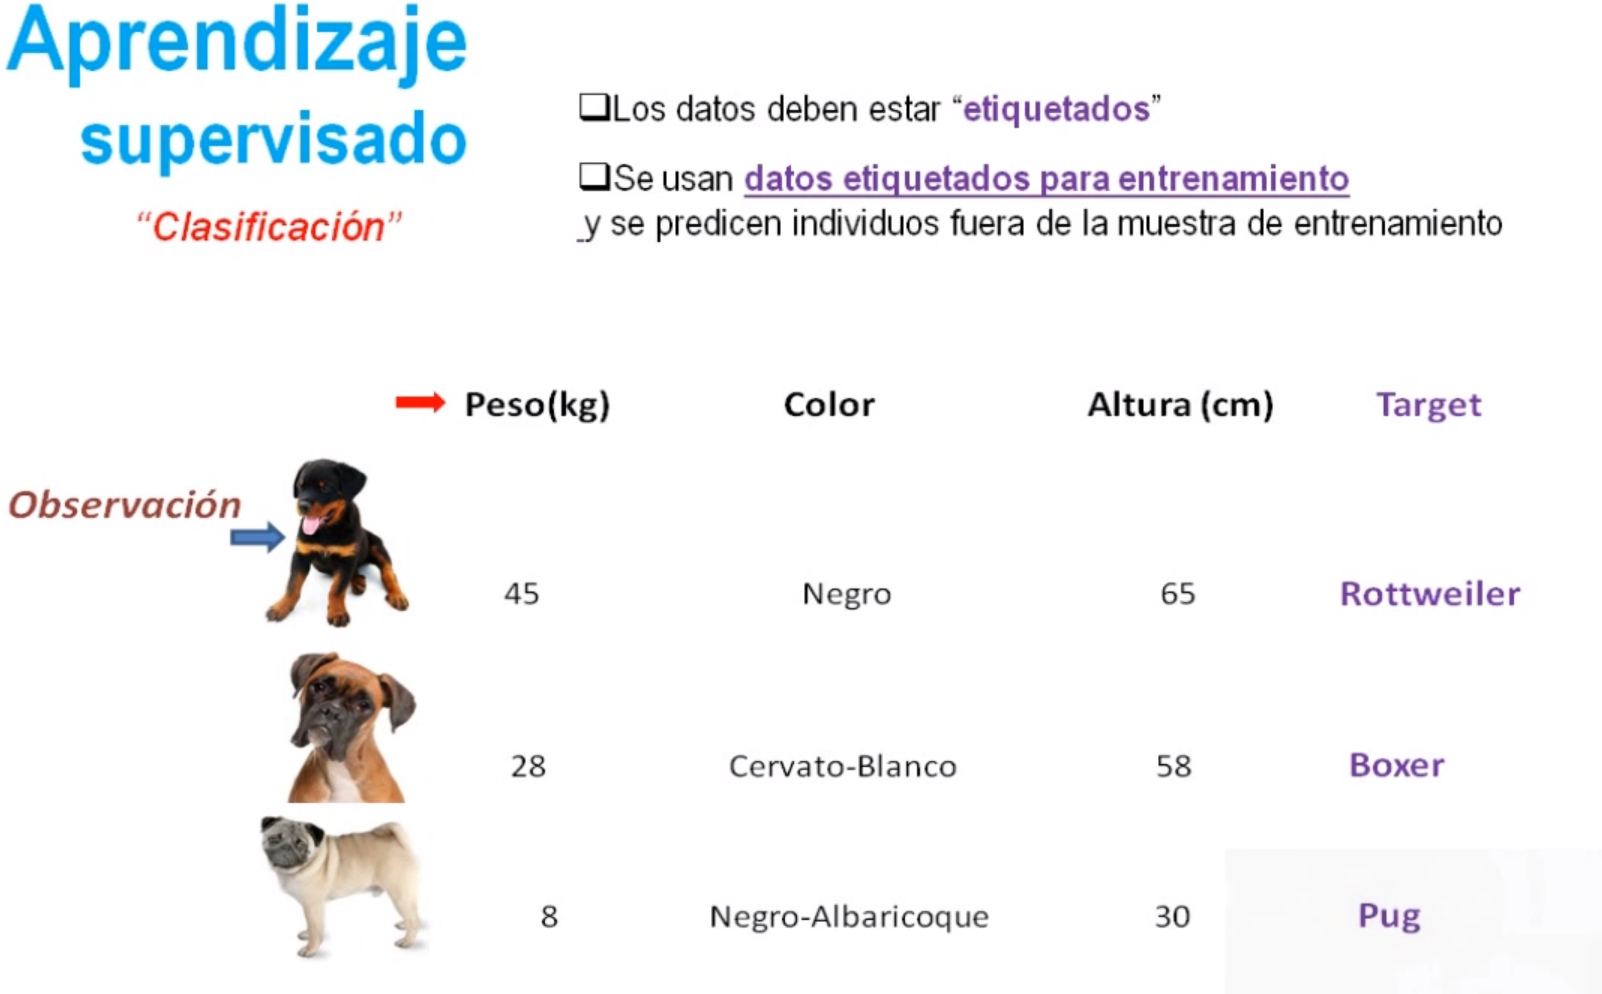
\includegraphics[width=7cm]{Imagenes/imagen1}

\end{itemize}



%----------------------------------------------------------------------------------------
%	BIBLIOGRAFIA
%----------------------------------------------------------------------------------------

\selectlanguage{spanish}
\begin{thebibliography}{99} 

\bibitem[1]{}
\newblock Gamma, Erich; Helm, Richard; Johnson, Ralph; Vlissides, John(1995).Design Patterns: Elements of Reusable Object- Oriented Software. Reading,Massachusetts: Addison Wesley Longman, Inc.



\end{thebibliography}


%----------------------------------------------------------------------------------------


\end{document}
